\documentclass[czech, 11pt]{article}

\usepackage{graphicx}
\usepackage[tmargin=25mm,bmargin=25mm,lmargin=25mm,rmargin=25mm]{geometry} %nastaveni okraju stranky
\usepackage[backend=biber, style=iso-numeric, alldates=iso]{biblatex} %citace
\usepackage[autostyle=true,czech=quotes]{csquotes} %\enquote
\usepackage[colorlinks=true,linkcolor=black,anchorcolor=black,citecolor=black,filecolor=black,menucolor=black,runcolor=black,urlcolor=black]{hyperref} %hypertextove odkazy v obsahu, color nutno nastavit aby kolem vsech odkazu nebyly barevne boxy
\usepackage[czech]{babel} %podpora pro cestinu
\usepackage{tabularx} %tabulky, potreba pro titulni stranu
\usepackage{datetime} %datum, potreba pro titulni stranu
\usepackage{enumitem} %\enumerate, \description, ...
\usepackage{listings} %vypisy kodu
\usepackage{xcolor} %barvy
\usepackage{amsmath} %matematika
\usepackage{caption} %captionof, ...
\usepackage{float}
\usepackage{parskip}
\usepackage{subfig}
\usepackage{todonotes}
\usepackage{pdflscape}

\newdateformat{kratkyDatum}{\THEDAY.\THEMONTH.\THEYEAR} %definovani formatu datumu, pro titulni stranu
\author{Boháčová Jana, Bc.; Keberle Ondřej, Bc.; Mlýnek Jakub, Bc.; Otava Michal, Bc.; Doubravský Ondřej, Bc.}
\addbibresource{citace.bib}
\graphicspath{{./Figures/}}



\renewcommand*\contentsname{Obsah} %zmena nadpisu obsahu
\renewcommand{\figurename}{Obrázek} %zmena nadpisu figure

\newcommand{\staticfigure}[3][1]{ %definice custom prikazu pro non-float obrazky
	%vlozi obrazek do textu a prida k nemu caption podobne jako figure, narozdil od figure to ale neni FLOAT! (tzn. tam kde vlozim command, tam zustane obrazek)
	%tri parametry, z toho jeden nepovinny:
	%scale (defaultne = 1), cesta k souboru, caption
	%pouziti:
	%napr. \staticfigure[0.7]{soubor.pdf}{Můj nejlepší obrázek}
	%nebo napr. \staticfigure{soubor.pdf}{Můj nejlepší obrázek}
	\noindent
	\begin{minipage}{\linewidth}
		\makebox[\linewidth]
		{
			\includegraphics[scale=#1]{#2}
		}
		\captionof{figure}{#3} 
	\end{minipage}
}




\begin{document}
	
	\begin{titlepage}
	\begin{center}
		\LARGE
		Vysoká škola báňská – Technická univerzita Ostrava\\
		Fakulta elektrotechniky a informatiky\\
		Katedra telekomunikační techniky
		
		\vspace*{1cm}
		
		
\includegraphics[]{feilogo.pdf}
		
		\Huge
		\textbf{Pokročilé síťové technologie II}
		
		\vspace{0.5cm}
		\Huge
		\textbf{Projekt}
		
		\vspace{1.5cm}
		
		\Huge
		Implementace adaptivního firewallu pomocí jazyka P4
		
		\vfill

		
		\vspace{0.8cm}
		
	\end{center}
    \vspace{0.8cm}
	\Large
    Vypracovali: Boháčová Jana, Keberle Ondřej, Mlýnek Jakub, Otava Michal, Doubravský Ondřej
	\begin{center}	
        \begin{tabularx}{\textwidth} { 
				 >{\raggedright\arraybackslash}X  
				 >{\raggedleft\arraybackslash}X  }
			      \\  & Datum: \kratkyDatum\today\\                 %TADY UPRAVIT LOGIN
			     Forma studia: prezenční & ak. r.: 2023/2024
		\end{tabularx}
	\end{center}

\end{titlepage} %titulni stranka
	\tableofcontents %obsah
	%\listoffigures %seznam figures
	%\listoftables %seznam tabulek
	\clearpage
	
	\section{Instalace prostředí}
    \todo[inline]{dopsat}
    
    citace tu \cite{p4vm}
	
	%\begin{figure}
	%	\centering
	%	\includegraphics[width=\textwidth,height=\textheight,keepaspectratio]{networksize-2021-11-08-2023-11-08.pdf}
	%	\caption{Testovací obrázek}
	%	\label{obrazek1}
	%\end{figure}
	
	%\subsection{Nadpis 2}
	%Test citace \cite{testCitace1} nebo \cite{testCitace2}.
	
	%\subsubsection{Nadpis 3}
	%Test odkaz na obrázek \ref{obrazek1}.

    \newpage
    \section{Popis struktury základního P4 programu - basic.p4}
    \todo[inline]{dopsat 2}
    \subsection{Headers}
    \subsection{Parser}
    \subsection{Checksum verification}
    \subsection{Ingress processing}
    \subsection{Egress processing}
    \subsection{Checksum computation}
    \subsection{Deparser}

    citace tu \cite{p4vm, dokumentace, p4prezentace}
    
    Popis kódu a funkce kódu v basic.p4 - dopsat
    Popis spuštění (make run) a vypnutí (make stop) - dopsat co se stane po spuštění příkazů make run(kompilace, spuštění kontroleru, spuštění tcpdump, spuštění mininetu, atd...) a make stop (vypne se to :D ale podrobněji popsat)
    
    \begin{figure}[H]
		\centering
		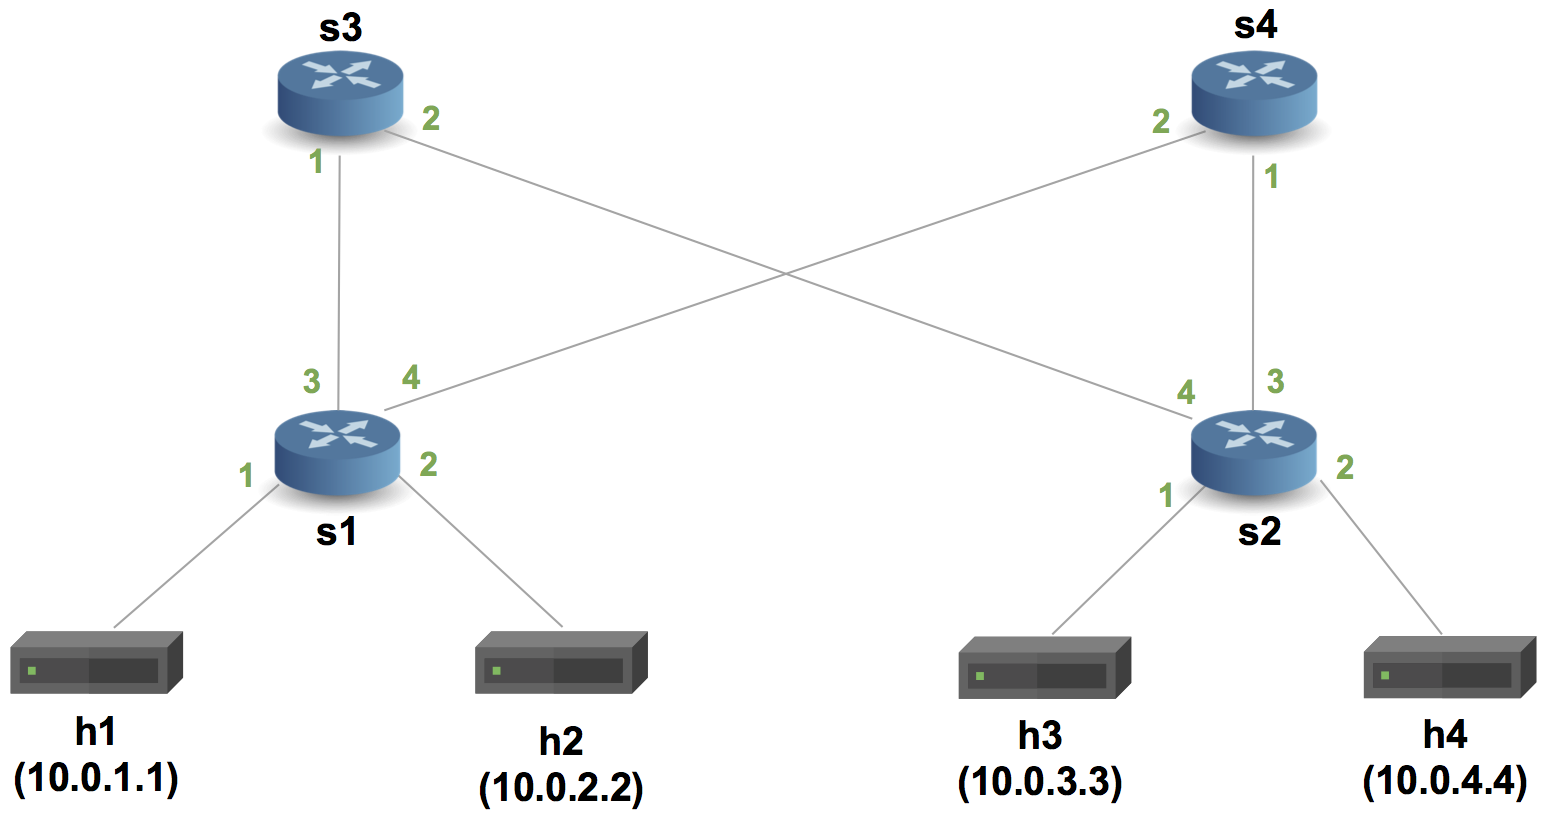
\includegraphics[width=\textwidth,height=\textheight,keepaspectratio]{pod-topo.png}
		\caption{Topologie příkladu basic.p4}
		\label{pod_topo}
	\end{figure}

    \todo[inline]{dopsat 2}
    dopsat kudma vedou cesty mezi jednotlivými hosty (viz. sX-runtime.json)


    \newpage
    \section{Implementace adaptivního firewallu}
    Hlavním cílem tohoto projektu, je vytvořit adaptivní firewall, který bude reagovat na ICMP packety, tj. na základě množství ICMP packetů za určitý časový interval, bude povolovat nebo blokovat provoz.
    \subsection{Základní počítání IPv4 packetů}
    \subsubsection{Úprava kódu}
    Prvním krokem bylo vyzkoušet, jakým způsobem P4 umožňuje počítat packety. K této funkcionalitě slouží v P4 konstrukce zvaná \textbf{counter}. Pro prvotní testování byla použita základní topologie, která byla vytvořena v příkladu \enquote{basic.p4}. P4 kód v této ukázce byl doplněn o countery počítající průchozí IPv4 packety skrz jednotlivé porty.

    V sekci \enquote{Ingress processing} programu jsme definovali nový counter nazvaný \enquote{port{\textunderscore}counter}. Tento counter je typu \enquote{packets{\textunderscore}and{\textunderscore}bytes}, počítá tedy jak packety tak byty.

    \begin{figure}[H]
		\centering
		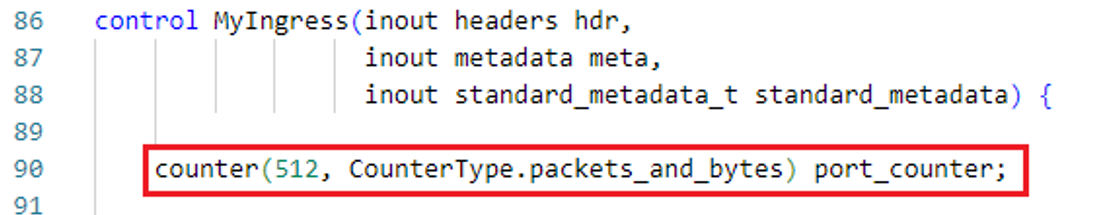
\includegraphics[width=.8\textwidth,height=\textheight,keepaspectratio]{port_counter.png}
		\caption{Definice nového counteru}
		\label{obrazek1}
	\end{figure}

    
    Níže v kódu jsme v akci \enquote{ipv4{\textunderscore}forward} přidali řádek s metodou \enquote{.count}, která zajišťovala samotné počítání packetů a bytů. Argumentem této metody je index (číslo) counteru, do kterého chceme hodnoty přičítat. V tomto případě je argumentem číslo portu, kterým packety prošli (standard{\textunderscore}metadata.ingress{\textunderscore}port). Tento řádek tedy počítá jednotlivé packety a byty na jednotlivých portech a ukládá tyto hodnoty do counterů indexovaných podle čísel portů (čísla portů viz. obrázek \ref{pod_topo}). \cite{cornell, dokumentace, bmv2simpleswitch, p4learning}
    \begin{figure}[H]
		\centering
		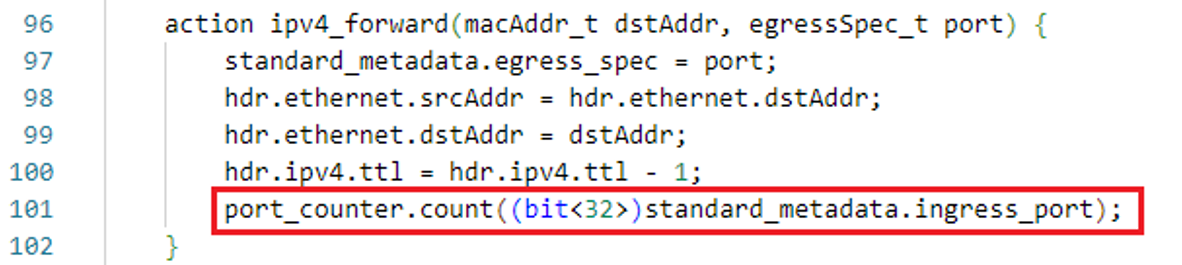
\includegraphics[width=.8\textwidth,height=\textheight,keepaspectratio]{action.png}
		\caption{Definice akce pro inkrementaci counteru}
		\label{obrazek2}
	\end{figure}

    
    \subsubsection{Čtení hodnot z counteru}
    Čtení hodnot z counteru lze nejjednodušším způsobem provádět pomocí tzv. \enquote{Runtime CLI}, což je utilita která umožňuje základní ovládání jednotlivých switchů pomocí příkazů.

    Každý switch v topologii dostane přidělen tzv. thrift port, pomocí kterého se k jednotlivým switchům připojíme. V testované topologie se jedná o porty 9090 - 9093 pro switche s1 - s4. Při otestování konektivity mezi hostem h1 a h3 příkazem ping, budou ICMP packety procházet sítí tak, jak je vyznačeno v obrázku \ref{pod_topo_counter_test}. Očekáváme tedy že se budou zvyšovat hodnoty counterů 1 a 3 na switchi s1, 1 a 2 na switchi s3 a 4 a 1 na switchi s2. Jednotlivé hodnoty counterů jsou zobrazeny na obr. \ref{counter_test}. \cite{runtimecli,bmv2simpleswitch,cornell}
    
    \begin{figure}[H]
		\centering
		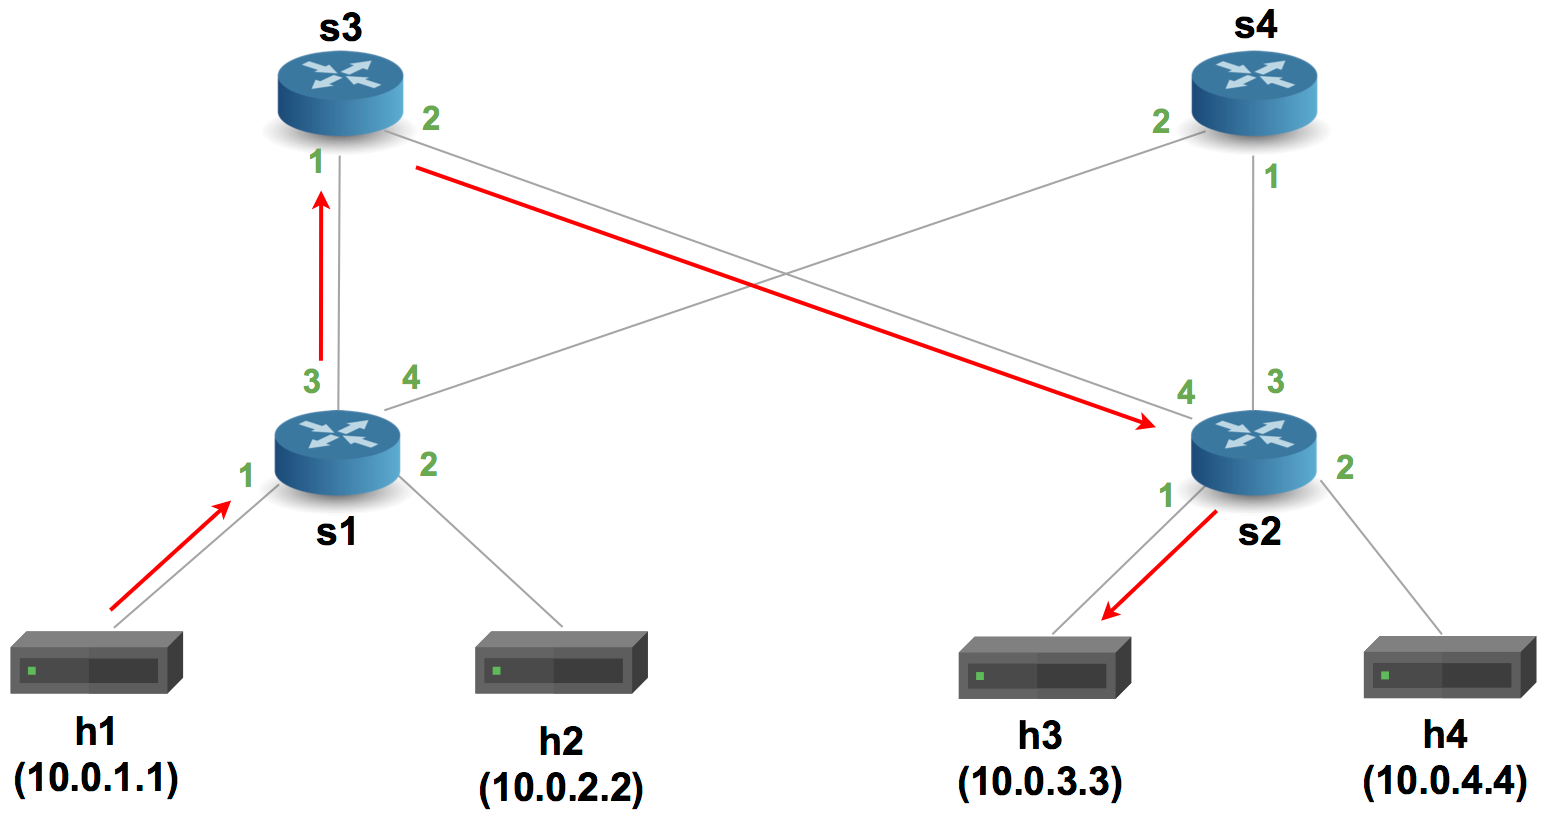
\includegraphics[width=0.75\textwidth,height=\textheight,keepaspectratio]{Figures/pod_topo_counter_test.png}
		\caption{Cesta packetů mezi h1 a h3}
		\label{pod_topo_counter_test}
	\end{figure}

    \begin{figure}[H]
        \centering
        \subfloat[s1]{{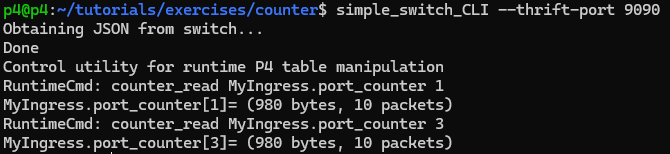
\includegraphics[width=0.75\textwidth]{s1.png} }}
        
        \subfloat[s2]{{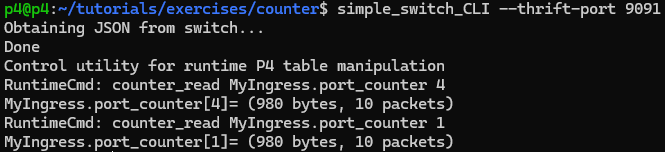
\includegraphics[width=0.75\textwidth]{s2.png} }}
        
        \subfloat[s3]{{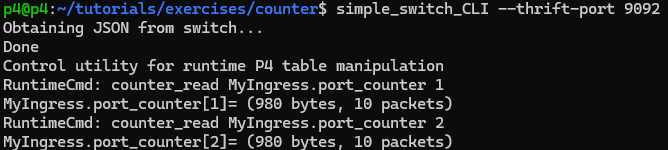
\includegraphics[width=0.75\textwidth]{s3.png} }}
        \caption{Test counterů}
        \label{counter_test}
    \end{figure}

    \subsection{Rozpoznávání ICMP packetů}
    Jelikož adaptivní firewall bude reagovat na ICMP packety, bylo další logickým krokem sestavit část programu, která bude odlišovat ICMP packety od ostatního provozu. Toto odlišení bylo provedeno na základě porovnávání hodnoty pole \enquote{protocol} v IPv4 záhlaví (obr. \ref{ip_header}), která je pro ICMP packety rovna 1 (viz. \cite{ip_protocols}). Do kódu bylo přidáno několik částí, které měli tuto klasifikaci provozu provádět. Jednalo se o \textbf{tabulku}, \textbf{akci} a \textbf{podmínku pro aplikování tabulky}.

     \begin{figure}[H]
		\centering
		
\includegraphics[width=.7\textwidth,height=\textheight,keepaspectratio]{Figures/ip_header.png}
		\caption{IP záhlaví}
		\label{ip_header}
	\end{figure}

    \begin{figure}[H]
		\centering
		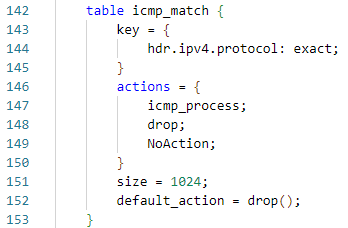
\includegraphics[width=.6\textwidth,height=\textheight,keepaspectratio]{icmp_table.png}
		\caption{Tabulka \enquote{icmp{\textunderscore}match}}
		\label{obrazek2}
	\end{figure}

     \begin{figure}[H]
		\centering
		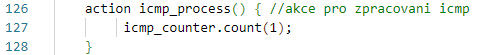
\includegraphics[width=.8\textwidth,height=\textheight,keepaspectratio]{icmp_action.png}
		\caption{Akce \enquote{icmp{\textunderscore}process}}
		\label{obrazek2}
	\end{figure}

     \begin{figure}[H]
		\centering
		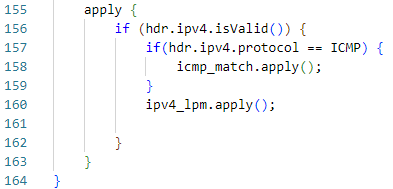
\includegraphics[width=.6\textwidth,height=\textheight,keepaspectratio]{apply_icmp_table.png}
		\caption{Podmínka pro aplikování tabulky \enquote{icmp{\textunderscore}match}}
		\label{obrazek2}
	\end{figure}

    Po přidání tohoto kódu a otestování pingem ale bohužel klasifikace ICMP nebyla funknčí, viz. logy na switchi s1.
    \begin{figure}[H]
		\centering
		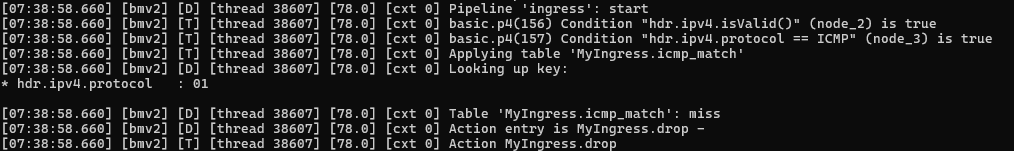
\includegraphics[width=\textwidth,height=\textheight,keepaspectratio]{logy_miss.png}
		\caption{Nefunkční klasifikace ICMP}
		\label{obrazek2}
	\end{figure}

    Ukázalo se, že toto je zapříčíněno způsobem, jakým jsou naplňovány tabulky jednotlivých switchů. Jelikož se jedná o základní ukázkový příklad, jsou jednotlivé záznamy definovány ručně, viz. níže, čímž. mj. odpadá nutnost řešit ARP.

    \begin{figure}[H]
		\centering
		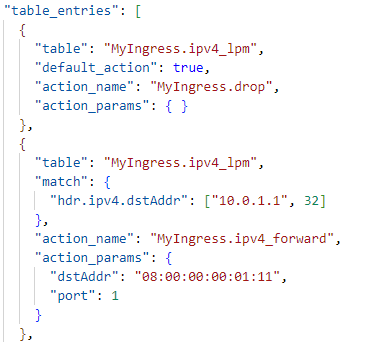
\includegraphics[width=.55\textwidth,height=\textheight,keepaspectratio]{Figures/tabulka_priklad.png}
		\caption{Příklad záznamů v tabulce}
		\label{obrazek2}
	\end{figure}

    Pro korektní identifikaci ICMP provozu bylo tedy nutné do tabulek všech switchů (soubor sX-runtime.json) vložit následující záznam.

    \begin{figure}[H]
		\centering
		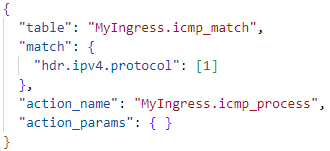
\includegraphics[width=.55\textwidth,height=\textheight,keepaspectratio]{Figures/icmp_zaznam.png}
		\caption{Záznam v tabulce pro zpracování ICMP}
		\label{obrazek2}
	\end{figure}

    Po tomto kroku se již akce definované v tabulce korektně spouštěly a tudíž počítání ICMP packetů bylo funknční, což dokazují obrázky níže.
    
    \subsubsection{Ověření funkčnosti}
    
    Na obrázku \ref{logy_hit} je zobrazen výpis logů, který ukazuje, že byla správně vyhodnocena sekvence klasifikace ICMP: 
    
    (hdr.ipv4.protocol == ICMP) $\rightarrow$ (icmp{\textunderscore}match) $\rightarrow$ (icmp{\textunderscore}process) $\rightarrow$ (icmp{\textunderscore}counter.count(...))

    \begin{figure}[H]
		\centering
		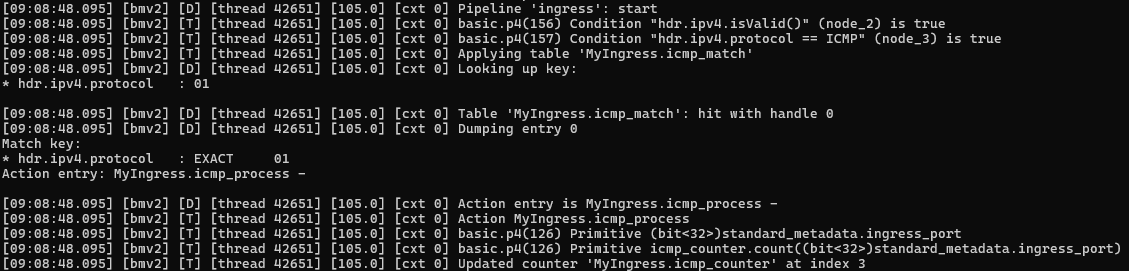
\includegraphics[width=\textwidth]{Figures/logy_hit.png}
		\caption{Funkční klasifikace ICMP}
		\label{logy_hit}
	\end{figure}

    Na obrázcích \ref{ping_test} a \ref{telnet_test} je poté zobrazeno otestování funkčnosti counterů. 
    
    Na obrázku \ref{ping_test}a) bylo provedeno 10 pingů, což odpovídá counterům na obrázku \ref{ping_test}b). Na tomto obrázku vidíme 20 ICMP packetů, což odpovídá 10 pingům (10 {$\cdot$} ECHO-REQUEST + 10 {$\cdot$} ECHO-REPLY).

    Na obrázku \ref{telnet_test}a) byl proveden test jiného provozu než ICMP (telnet), což se v counterech (obrázek \ref{telnet_test}b)) projevilo přičtením jednoho packetu do port{\textunderscore}counteru, ale nikoliv do icmp{\textunderscore}counteru. Počítání ICMP packetů tedy funguje správně.

    \begin{figure}[H]
        \centering
        \subfloat[ping]{{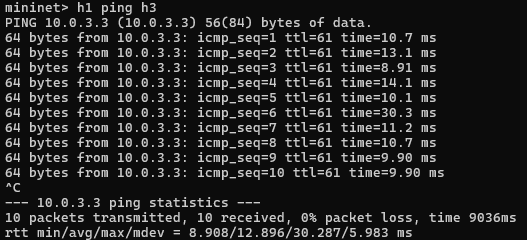
\includegraphics[]{Figures/pocitani_ping/ping.png}}}
        
        \subfloat[Hodnoty counterů]{{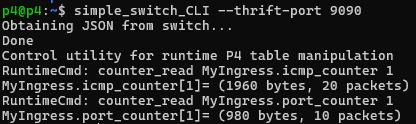
\includegraphics[]{Figures/pocitani_ping/counter_pred_telnetem.png}}}
        \caption{Test počítání ICMP packetů - ping}
        \label{ping_test}
    \end{figure}

    \begin{figure}[H]
        \centering
        \subfloat[telnet]{{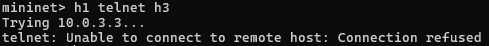
\includegraphics[]{Figures/pocitani_ping/telnet.png}}}
        
        \subfloat[Hodnoty counterů]{{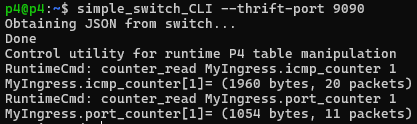
\includegraphics[]{Figures/pocitani_ping/counter_po_telnetu.png}}}
        \caption{Test počítání ICMP packetů - telnet}
        \label{telnet_test}
    \end{figure}

    \newpage
    \subsubsection{Odlišení REQUEST a REPLY zpráv}
    Jelikož nechceme duplicitní hodnoty počtu pingů, bylo nutné odlišit REQUEST a REPLY zprávy. Toto odlišení bylo provedeno na základě porovnávání hodnoty \enquote{code} uvnitř ICMP záhlaví (obr. \ref{icmp_header}), která je pro REQUEST zprávy = 8 a pro REPLY = 0 (viz. \cite{icmpmessages}).

    \begin{figure}[H]
		\centering
		
\includegraphics[width=.6\textwidth,height=\textheight,keepaspectratio]{Figures/icmp_header.png}
		\caption{ICMP záhlaví}
		\label{icmp_header}
	\end{figure}

    Abychom se k tomuto poli dostali, potřebovali jsme parsovat ICMP záhlaví. Do P4 kódu bylo tedy dodáno: definice ICMP záhlaví, ICMP parser, podmínka pro odlišení REQUEST a REPLY zpráv, Deparser.

    \begin{figure}[H]
		\centering
		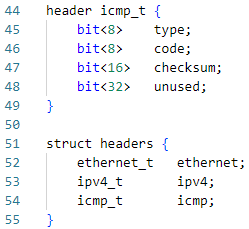
\includegraphics[width=.3\textwidth,height=\textheight,keepaspectratio]{Figures/icmp_parsovani/header.png}
		\caption{Definice ICMP záhlaví}
		\label{icmp_header}
	\end{figure}

    \begin{figure}[H]
		\centering
		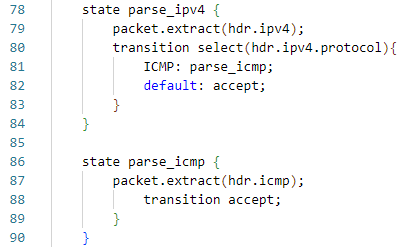
\includegraphics[width=.5\textwidth,height=\textheight,keepaspectratio]{Figures/icmp_parsovani/parser.png}
		\caption{ICMP parser}
		\label{icmp_header}
	\end{figure}

     \begin{figure}[H]
		\centering
		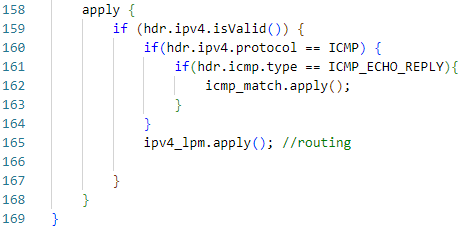
\includegraphics[width=.6\textwidth,height=\textheight,keepaspectratio]{Figures/icmp_parsovani/apply.png}
		\caption{Odlišení REQUEST a REPLY zpráv}
		\label{icmp_header}
	\end{figure}

     \begin{figure}[H]
		\centering
		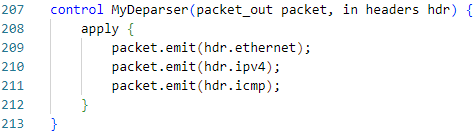
\includegraphics[width=.6\textwidth,height=\textheight,keepaspectratio]{Figures/icmp_parsovani/deparser.png}
		\caption{Deparser}
		\label{icmp_header}
	\end{figure}

    V tomto stavu bylo funknčí počítání pouze ICMP ECHO-REPLY zpráv.
    
    \subsection{Implementace kontroleru}
    Dalším krokem bylo implementace kontroleru, který bude rozhodovat o povolení/zablokování provozu. Kostra Python kódu pro kontroler byla převzata z ukázkového kódu \enquote{p4runtime}, ze kterého jsme použili funkce \enquote{printCounter}, \enquote{readTableRules}, \enquote{printGrpcError} a \enquote{main}, do kterého jsme později doplnili další funkce.

    \subsubsection{Komunikace kontroleru se switchem}
    \todo[inline]{dopsat 3}
    TEORIE... dopsat jak komunikujou switche s kontrolerem (pomocí P4RUNTIME (co to je atd, gRPC porty, ...)
    

    \newpage
    \subsubsection{Základní kostra kontroleru, vyčítání hodnot counterů}
    Základem kontroleru je metoda \enquote{main}. V této metodě provádíme v základní podobě následující akce: 
    \begin{itemize}
        \item navázání spojení k jednotlivým switchům
        \item odeslání \enquote{master arbitration update} zpráv
        \item vyčtení záznamů tabulek z jednotlivých switchů
        \item vyčítání požadovaných counterů co 2 sek.
    \end{itemize}

    Kód metody \enquote{main} je zobrazen na obr. \ref{main}. Ukázkový výpis vyčítání counterů je zobrazen na obr. \ref{controller_counter_read}
    \begin{figure}[H]
		\centering
		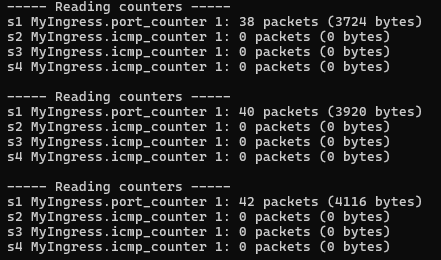
\includegraphics[width=.7\textwidth]{Figures/controller/vycitani_counteru_priklad.png}
		\caption{Vyčítání counterů pomocí kontroleru}
		\label{controller_counter_read}
	\end{figure}
    

    \begin{figure}[H]
		\centering
		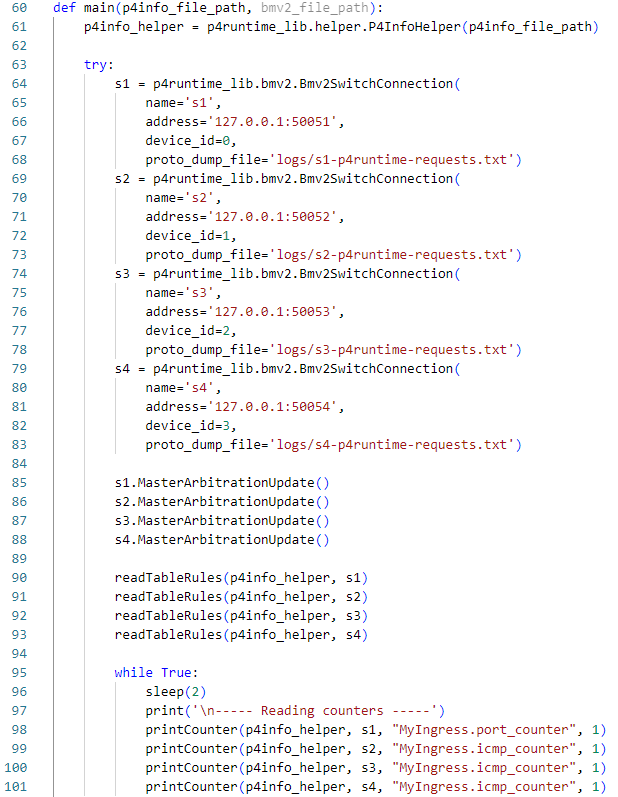
\includegraphics[width=\textwidth]{Figures/controller/metoda_main.png}
		\caption{Metoda \enquote{main}}
		\label{main}
	\end{figure}

    \subsubsection{Funkcionalita pro manipulaci s tabulkama}
    Aby bylo možné povolovat nebo zakazovat provoz, bylo potřeba zajistit způsob, jakým bychom mohli přidávat nebo odebírat pravidla z tabulek.

    Pro přidávání pravidla slouží funkce \enquote{writeIpForwardRule}, která na základě předaných parametrů přidá nové pravidlo do tabulky \enquote{ipv4{\textunderscore}lpm}.

    \begin{figure}[H]
		\centering
		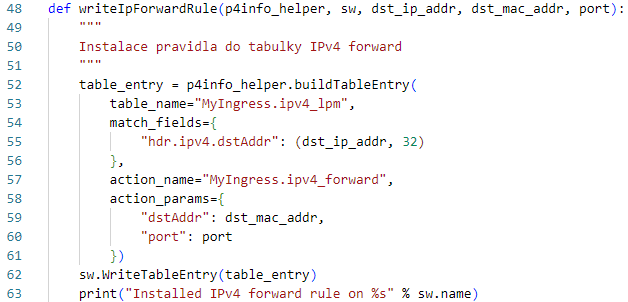
\includegraphics[width=.9\textwidth]{Figures/controller/writeipforwardrule.png}
		\caption{writeIpForwardRule}
		\label{...}
	\end{figure}

    Pro odebírání pravidel z tabulky slouží funkce \enquote{deleteIpForwardRule}, která na základě předaných parametrů odstraní pravidlo z tabulky \enquote{ipv4{\textunderscore}lpm}. Tato funkce závisí na funkci switche \enquote{DeleteTableEntry}, která není ve switchi defaultně implementovaná, tudíž ji bylo nutné do souboru \enquote{utils/p4runtime{\textunderscore}lib/switch.py} dodat.

    \begin{figure}[H]
		\centering
		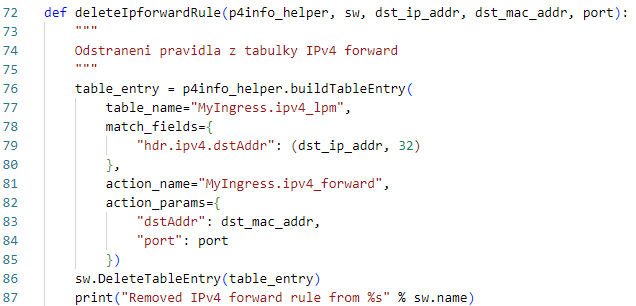
\includegraphics[width=.9\textwidth]{Figures/controller/deleteipforwardrule.png}
		\caption{deleteIpForwardRule}
		\label{...}
	\end{figure}

    \subsubsection{Implementace logiky blokování/povolování provozu}
    Logika adaptivního firewallu spočívá v počítání ICMP (ECHO-REPLY) packetů procházející switchi s1 a s2. V případě že na daném switchi překročí počet těchto packetů práhovou hodnotu (defaultně 10) za určitý čas (defaultně 10s), odstraní se z tabulky na daném switchi pravidla pro IP směrování na portech 1 a 2. Zároveň se nastaví proměnná \enquote{sX{\textunderscore}blocked{\textunderscore}flag} na hodnotu True, abychom zamezili pokusům o mazání pravidel, které již na switchi neexistují.

    Pokud hodnota průchozích packetů později klesne pod mez, pravidla pro směrování se opět nainstalují (čímž se opětovně povolí provoz) a proměnná \enquote{sX{\textunderscore}blocked{\textunderscore}flag} se nastaví na False.

    Toto rozhodování probíhá v nekonečné smyčce.

    \bigskip
    \bigskip

    Tuto funkci ověříme např. příkazem ping s parametrem -i. Tento parametr nastavuje interval mezi jednolivými odeslanými ECHO-REQUEST zprávami. Například příkazem ping -i 0.5 vyšleme 2 packety za sekundu, čímž zablokujeme provoz. Po uplynutí 10s se provoz znovu povolí, za 10s znovu zablokuje, atd...

    \begin{figure}[H]
		\centering
		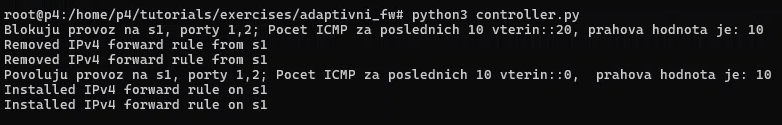
\includegraphics[width=\textwidth]{Figures/controller/funkcni.png}
		\caption{Ukázka funkce controlleru}
		\label{...}
	\end{figure}

    \begin{landscape}
         \begin{figure}
            \centering
		      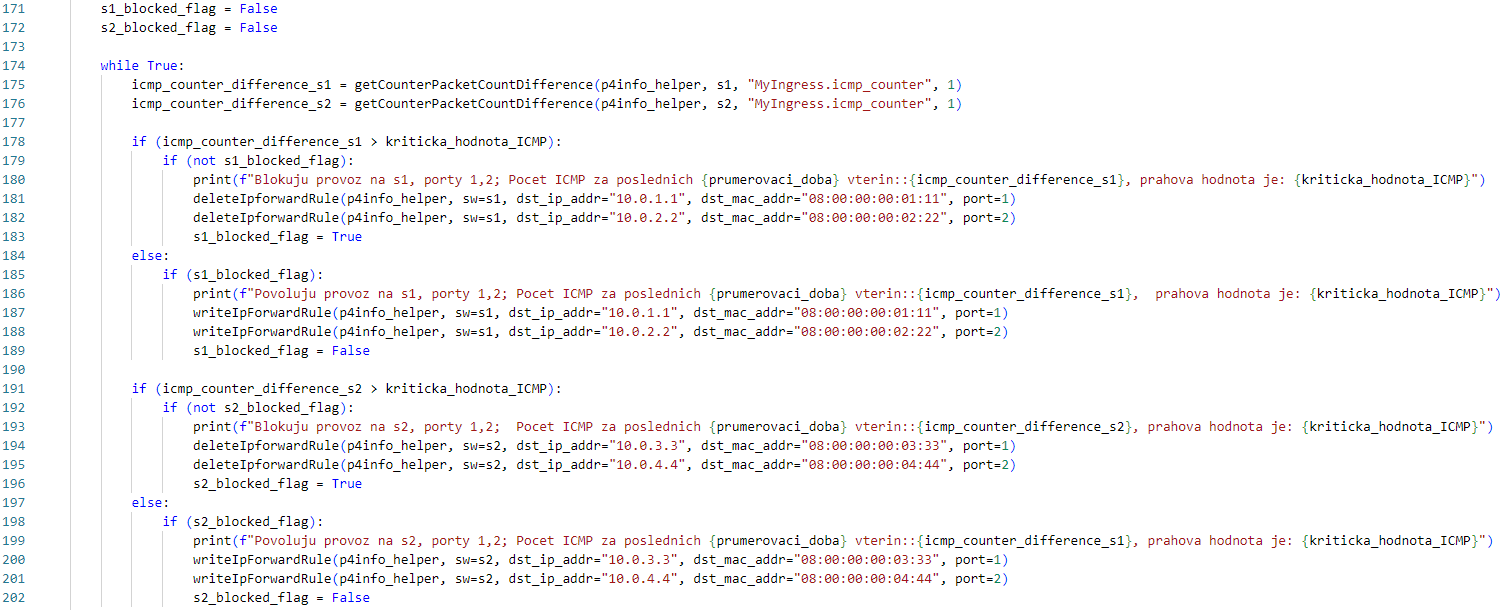
\includegraphics[scale=0.6]{Figures/controller/logika.png}
		      \caption{Blokování/povolování provozu}
		      \label{...}
         \end{figure}
    \end{landscape}

    \section{Závěr}
    \todo[inline]{dopsat 4}
    
    
	\clearpage
	\printbibliography[title={Literatura}, heading=bibintoc] %seznam literatury
\end{document}